% =====================================================================
%  IN6049 --- Forecasting and Regression Analysis
%  Week 5: Multiple Regression II and Quantitative/Qualitative Predictors --- Tips dataset
%
%  Built from template/slides-template.tex (Boadilla + seahorse, 16:9).
%  Title slide + 9 content slides.  Numbers come from Assigment_5.ipynb;
%  figures are its exported PNGs (images/ -> fig_*.png here).
%
%  Compiles on Overleaf with the default pdfLaTeX engine.
%  Upload alongside: fig_bands.png , fig_plane.png , fig_stab.png , fig_poly.png ,
%  fig_inter.png , fig_par.png , fig_smoker.png
% =====================================================================
\documentclass[aspectratio=169,11pt]{beamer}

\usetheme{Boadilla}
\usecolortheme{seahorse}
\setbeamertemplate{navigation symbols}{}

\usepackage[utf8]{inputenc}
\usepackage[T1]{fontenc}
\usepackage{booktabs}
\usepackage{amsmath}
\usepackage{graphicx}
\usepackage{url}

% Emphasis lead-in: bold + structure colour.  Use as \key{Finding.} text...
\newcommand{\key}[1]{\textbf{\structure{#1}}}

% Figure placeholder, so the template compiles with no image files.
% Replace each use by  \includegraphics[width=0.9\linewidth]{@@ file @@}
% (vector PDF preferred; PNG is fine).
\newcommand{\figbox}[2]{%
  \fbox{\parbox[c][#2][c]{#1}{\centering\scriptsize\color{gray}@@ figure @@}}}

% ---------------------------------------------------------------------
\title[Multiple regression II, indicators]{Multiple Regression II and Indicator Variables --- Tips}
\subtitle{Partial tests, multicollinearity, polynomial and qualitative predictors}
\author[Jie Dong, Elivier Reyes]{Jie Dong, Elivier Reyes}
\date[IN6049]{}

\begin{document}

% ===================== TITLE ========================================
\begin{frame}
  \titlepage
  \vspace{-1.2em}
  \begin{center}
    \small\urlstyle{same}\url{https://github.com/HelloJJJie/Assignment-Forecast-and-Analysis-of-Regression.git}

    \vspace{1.2em}
    $n=244$ restaurant bills --- which predictors of the tip are \emph{needed}, what happens
    when they overlap, and do groups differ?
  \end{center}
\end{frame}

% ===================== RECAP 1: SIMPLE REGRESSION ===================
\begin{frame}{1. Recap: simple linear regression (weeks 1--3)}
  \begin{columns}[T]
  \begin{column}{0.52\textwidth}
    \small
    \key{Model.} $\hat Y=0.920+0.105\,X$ ($X=$ bill, $Y=$ tip, $n=244$).

    \vspace{0.3em}
    {\scriptsize
    \begin{tabular}{@{}lr@{\hskip 1.2em}lr@{}}
      \toprule
      $b_1$      & $0.1050$ & $R^2$    & $0.457$ \\
      $s\{b_1\}$ & $0.0074$ & $r$      & $0.676$ \\
      $95\%$ CI  & $[0.0905,\,0.1195]$ & $s$ & $1.02$ \\
      $t^{*}$    & $14.26$  & $F^{*}$  & $203.4$ \\
      \bottomrule
    \end{tabular}}

    \vspace{0.3em}
    \begin{itemize}
      \item \key{Diagnostics:} constant variance rejected (Brown--Forsythe
            $P=1.4\times10^{-7}$, Breusch--Pagan $P=4\times10^{-21}$); normality
            rejected ($r=0.982$ vs.\ $0.994$); $5$ cases with $|e^{*}|>3$.
      \item \key{Simultaneous inference:} a family $95\%$ interval for
            $\beta_0,\beta_1$ needs multiplier $2.255$ (Bonferroni), not
            $1.970$; the whole-line band uses $W=2.463$.
    \end{itemize}
  \end{column}
  \begin{column}{0.48\textwidth}
    \centering
    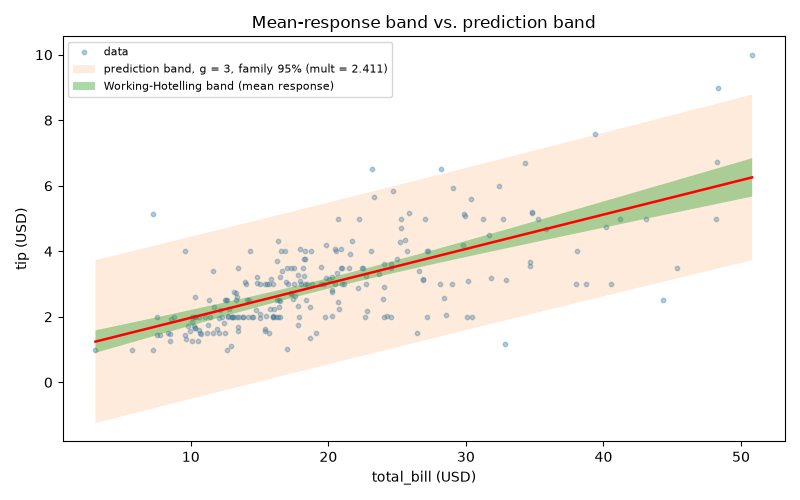
\includegraphics[width=0.84\linewidth]{fig_bands.png}

    \vspace{-0.1em}
    {\scriptsize Prediction band ($g=3$) vs.\ Working--Hotelling band: the new-tip
     band is about $15\times$ wider at $\bar X$.}
  \end{column}
  \end{columns}
\end{frame}

% ===================== RECAP 2: MULTIPLE REGRESSION =================
\begin{frame}{2. Recap: multiple regression and the hat matrix (week 4)}
  \begin{columns}[T]
  \begin{column}{0.52\textwidth}
    \small
    \key{Model.} $\hat Y=0.669+0.0927X_1+0.1926X_2$ ($X_2=$ party size).

    \vspace{0.3em}
    {\scriptsize
    \begin{tabular}{@{}lrrr@{}}
      \toprule
       & $b$ & $s\{b\}$ & $t^{*}$ \\
      \midrule
      total bill & $0.0927$ & $0.0091$ & $10.17$ \\
      size       & $0.1926$ & $0.0853$ & $2.26$ \\
      \bottomrule
    \end{tabular}}

    \vspace{0.3em}
    \begin{itemize}
      \item \key{Fit:} $F^{*}=105.95$, $R^2=0.468$, $R^2_a=0.463$ --- only
            $0.011$ above the bill alone.
      \item \key{Hat matrix:} $\mathbf H$ symmetric, idempotent,
            $\operatorname{tr}\mathbf H=p$; $22$ of $244$ cases have
            $h_{ii}>2p/n$.
      \item \key{Influence:} row $170$ (bill \$50.81): leverage $0.071$,
            $r=4.14$, Cook's $D=0.437$; dropping the top three cases moves
            the coefficients $12$--$19\%$.
    \end{itemize}
  \end{column}
  \begin{column}{0.48\textwidth}
    \centering
    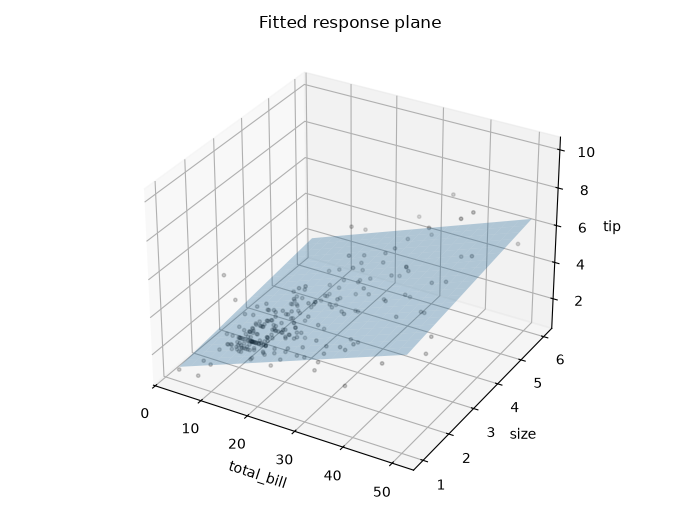
\includegraphics[width=0.88\linewidth]{fig_plane.png}

    \vspace{-0.1em}
    {\scriptsize Each coefficient holds the other predictor fixed. Variance is
     still not constant (Breusch--Pagan $\chi^2=92.2$).}
  \end{column}
  \end{columns}
\end{frame}

% ===================== 1. EXTRA SS AND PARTIAL F ====================
\begin{frame}{3. Extra sums of squares and partial $F$ tests}
  \begin{columns}[T]
  \begin{column}{0.50\textwidth}
    \small
    $Y=$ tip, $X_1=$ bill, $X_2=$ size, $X_3=$ bill per person ($X_1/X_2$).

    \vspace{0.2em}
    $SSR(X_2\mid X_1)=SSE(X_1)-SSE(X_1,X_2)$: the extra error removed by
    adding $X_2$. \key{The order matters:}

    \vspace{0.3em}
    {\scriptsize
    \begin{tabular}{@{}lrlr@{}}
      \toprule
      \multicolumn{2}{c}{order $X_1,X_2,X_3$} & \multicolumn{2}{c}{order $X_3,X_2,X_1$} \\
      \midrule
      $SSR(X_1)$          & $212.42$ & $SSR(X_3)$          & $56.14$ \\
      $SSR(X_2\mid X_1)$  & $5.24$   & $SSR(X_2\mid X_3)$  & $145.32$ \\
      $SSR(X_3\mid X_1,X_2)$ & $1.30$ & $SSR(X_1\mid X_3,X_2)$ & $17.50$ \\
      \midrule
      sum                 & $218.96$ & sum                 & $218.96$ \\
      \bottomrule
    \end{tabular}}

    \vspace{0.4em}
    Both orders add up to the same $SSR=218.96$ of $SSTO=465.21$.
  \end{column}
  \begin{column}{0.50\textwidth}
    \small
    \key{Partial $F$, one coefficient} ($F^{*}=(t^{*})^2$; $F(0.95;1,240)=3.88$):

    \vspace{0.2em}
    {\scriptsize
    \begin{tabular}{@{}lrrr@{}}
      \toprule
       & $F^{*}$ & $t^{*}$ & $P$ \\
      \midrule
      total bill & $17.05$ & $+4.13$ & $5.0\times10^{-5}$ \\
      size       & $0.03$  & $-0.16$ & $0.87$ \\
      per person & $1.27$  & $-1.13$ & $0.26$ \\
      \bottomrule
    \end{tabular}}

    \vspace{0.4em}
    \key{A pair at once} ($F(0.95;2,240)=3.03$):

    \vspace{0.2em}
    {\scriptsize
    \begin{tabular}{@{}lrr@{}}
      \toprule
      Dropped together & $F^{*}$ & $P$ \\
      \midrule
      size + per person       & $3.19$  & $0.043$ \\
      bill + per person       & $52.4$  & $1.3\times10^{-19}$ \\
      bill + size             & $79.3$  & $3.6\times10^{-27}$ \\
      \bottomrule
    \end{tabular}}

    \vspace{0.4em}
    Given the others, only the bill is needed --- yet size and per-person
    \emph{together} are borderline significant.
  \end{column}
  \end{columns}
\end{frame}

% ===================== 2. PARTIAL R2, STANDARDIZED, VIF =============
\begin{frame}{4. Partial $R^2$, standardization, multicollinearity}
  \begin{columns}[T]
  \begin{column}{0.46\textwidth}
    \small
    \key{Partial $R^2$} (share of what the others leave that a predictor explains):

    \vspace{0.2em}
    {\scriptsize
    \begin{tabular}{@{}lrr@{}}
      \toprule
       & $R^2$ partial & partial $r$ \\
      \midrule
      $R^2_{Y2|1}$   & $0.0207$ & $+0.144$ \\
      $R^2_{Y3|12}$  & $0.0053$ & $-0.073$ \\
      $R^2_{Y1|23}$  & $0.0663$ & $+0.258$ \\
      \bottomrule
    \end{tabular}}

    \vspace{0.4em}
    \key{Correlation transform} ($\mathbf r_{XX}\mathbf b^{*}=\mathbf r_{YX}$):

    \vspace{0.2em}
    {\scriptsize
    \begin{tabular}{@{}lrrr@{}}
      \toprule
       & $b_k$ & $s_k$ & $b^{*}_k$ \\
      \midrule
      total bill & $0.1253$  & $8.90$ & $+0.806$ \\
      size       & $-0.0356$ & $0.95$ & $-0.024$ \\
      per person & $-0.0850$ & $2.91$ & $-0.179$ \\
      \bottomrule
    \end{tabular}}

    \vspace{0.2em}
    {\small Condition number $49{,}234$ for $X'X$ vs.\ $67.8$ for $\mathbf r_{XX}$.}
  \end{column}
  \begin{column}{0.54\textwidth}
    \centering
    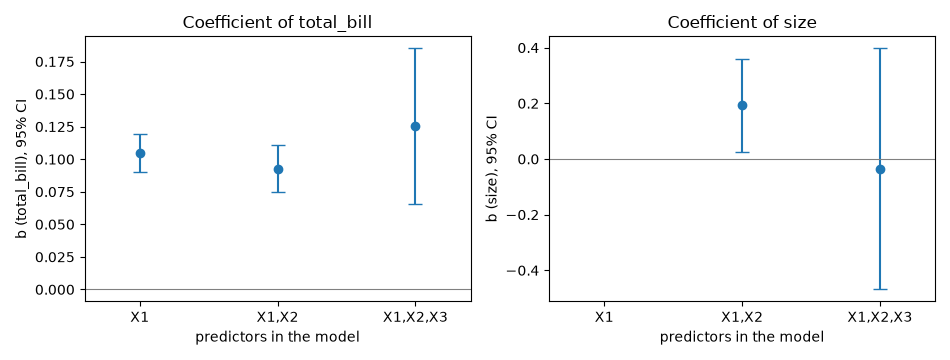
\includegraphics[width=0.96\linewidth]{fig_stab.png}

    \vspace{0.1em}
    \raggedright\small
    \key{Unstable and imprecise:} the size coefficient flips from $+0.193$ to
    $-0.036$ when per person (derived: $X_1/X_2$) enters; $s\{b_1\}$ grows
    $4.1\times$.

    \vspace{0.2em}
    \key{VIF} $=17.3,\ 10.4,\ 11.4$ ($1.56$ without per person). Still fine:
    $R^2$ $0.468\to0.471$, prediction at (\$20, party of 3) $3.10\to3.11$.\par
  \end{column}
  \end{columns}
\end{frame}

% ===================== 5. POLYNOMIAL ================================
\begin{frame}{5. Polynomial regression and centering}
  \begin{columns}[T]
  \begin{column}{0.50\textwidth}
    \small
    \key{Second-order model} with the centered predictor $x=X-\bar X$:
    \[ Y=\beta_0+\beta_1x+\beta_{11}x^2+\varepsilon \]
    Still linear in the $\beta$'s, so ordinary least squares applies.

    \vspace{0.3em}
    \begin{itemize}
      \item \key{Why center:} $X$ and $X^2$ are strongly correlated over a
            positive range; centering makes $X'X$ better conditioned.
      \item \key{Back to the original scale:} $b_1=b_1'-2b_{11}'\bar X$,
            $b_0=b_0'-b_1'\bar X+b_{11}'\bar X^2$ (checked against the raw fit).
      \item \key{Test the curvature:} $t^{*}=-0.09$, $P=0.92$; $R^2_a$
            $0.4544\to0.4521$. The fitted curve lies on the line.
    \end{itemize}
  \end{column}
  \begin{column}{0.50\textwidth}
    \centering
    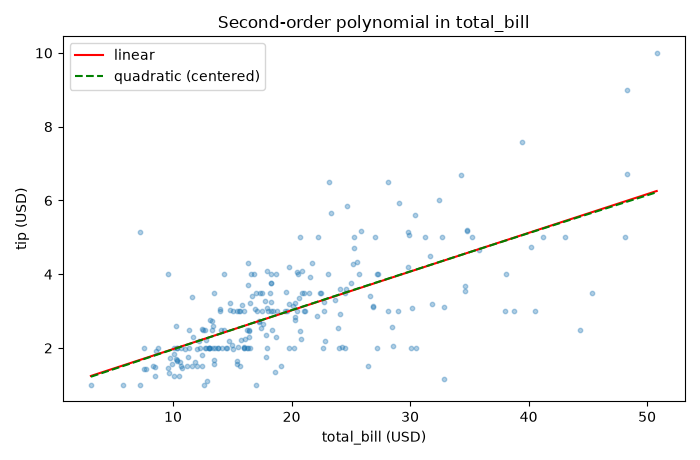
\includegraphics[width=0.88\linewidth]{fig_poly.png}

    \vspace{0.3em}
    {\scriptsize
    \begin{tabular}{@{}lrr@{}}
      \toprule
       & raw $X$ & centered $x$ \\
      \midrule
      $\mathrm{corr}(X,X^2)$ & $0.971$ & $0.633$ \\
      cond.\ number of $X'X$ & $1.2\times10^{7}$ & $4.0\times10^{4}$ \\
      \bottomrule
    \end{tabular}}

    \vspace{0.2em}
    {\scriptsize Not $0$: the bill is right-skewed (skewness $1.13$); it is exactly $0$ only for symmetric $X$.}
  \end{column}
  \end{columns}
\end{frame}

% ===================== 6. INTERACTION ===============================
\begin{frame}{6. Interaction between two quantitative predictors}
  \begin{columns}[T]
  \begin{column}{0.50\textwidth}
    \small
    \key{Interaction:} $E\{Y\}=\beta_0+\beta_1X_1+\beta_2X_2+\beta_3X_1X_2$;
    the slope in the bill is $\beta_1+\beta_3X_2$. Additive $\Rightarrow$ parallel,
    interacting $\Rightarrow$ not parallel.

    \vspace{0.3em}
    {\scriptsize
    \begin{tabular}{@{}rcc@{}}
      \toprule
      party size & slope of the bill & $95\%$ CI \\
      \midrule
      $1$ & $0.0858$ & $[0.0545,\,0.1172]$ \\
      $3$ & $0.0937$ & $[0.0753,\,0.1121]$ \\
      $6$ & $0.1055$ & $[0.0545,\,0.1565]$ \\
      \bottomrule
    \end{tabular}}

    \vspace{0.3em}
    \begin{itemize}
      \item $b_3=+0.0039$, $t^{*}=0.53$, $P=0.60$: no evidence of interaction.
      \item \key{Full second-order model} (5 terms): none of $x_1^2$, $x_2^2$,
            $x_1x_2$ is significant; together $F^{*}=0.24$, $P=0.87$;
            $R^2_a$ $0.4635\to0.4583$.
    \end{itemize}
  \end{column}
  \begin{column}{0.50\textwidth}
    \centering
    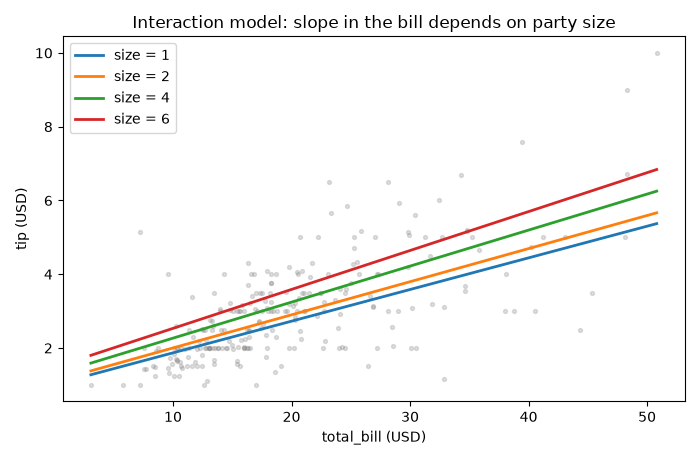
\includegraphics[width=0.90\linewidth]{fig_inter.png}

    \vspace{-0.1em}
    {\scriptsize The lines for party sizes $1,2,4,6$ are nearly parallel.}

    \vspace{0.3em}
    \raggedright\small
    \key{So:} for bill and size the additive first-order model is enough.\par
  \end{column}
  \end{columns}
\end{frame}

% ===================== 7. INDICATORS ================================
\begin{frame}{7. Qualitative predictors: indicator variables}
  \begin{columns}[T]
  \begin{column}{0.50\textwidth}
    \small
    \key{Coding.} A class has no scale: use $0/1$ indicators.
    $\mathbf{c-1}$ \key{for $c$ classes} --- with $c$ indicators plus the intercept,
    $\mathbf X'\mathbf X$ is singular. The all-zero class is the baseline.

    \vspace{0.3em}
    \key{Parallel lines} ($Z=1$ for smokers):
    \[ \hat Y=0.963+0.1057X_1-0.149\,Z \]
    $b_2=-0.149$, $95\%$ CI $[-0.415,\,0.117]$, $P=0.27$: no vertical shift.

    \vspace{0.3em}
    \key{\texttt{day}} has $4$ classes: intercept $+$ $4$ indicators has rank $4$ of $5$.
  \end{column}
  \begin{column}{0.50\textwidth}
    \centering
    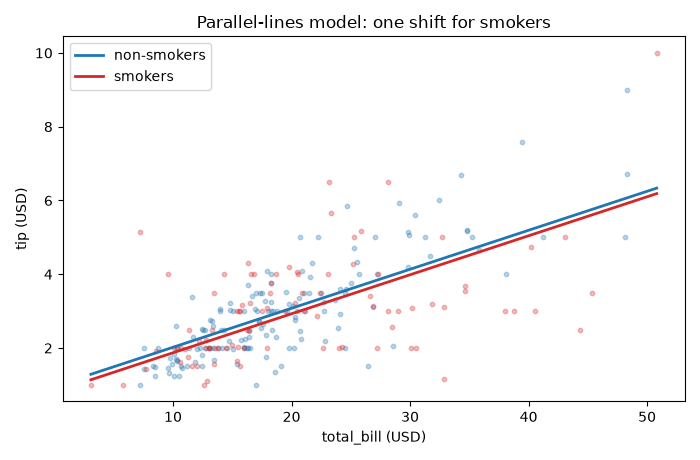
\includegraphics[width=0.84\linewidth]{fig_par.png}

    \vspace{0.3em}
    {\scriptsize
    \begin{tabular}{@{}lrrrr@{}}
      \toprule
      baseline & Fri & Sat & Sun & Thur \\
      \midrule
      Fri  & --       & $-0.086$ & $+0.075$ & $-0.019$ \\
      Sat  & $+0.086$ & --       & $+0.161$ & $+0.067$ \\
      Thur & $+0.019$ & $-0.067$ & $+0.094$ & -- \\
      \bottomrule
    \end{tabular}}

    \vspace{0.2em}
    {\scriptsize Each row: shift of the column's day relative to the baseline. Same
     fit for every baseline (SSE $251.74$).}
  \end{column}
  \end{columns}
\end{frame}

% ===================== 8. COMPARING FUNCTIONS =======================
\begin{frame}{8. Comparing regression functions: smokers vs.\ non-smokers}
  \begin{columns}[T]
  \begin{column}{0.52\textwidth}
    \small
    $E\{Y\}=\beta_0+\beta_1X_1+\beta_2Z+\beta_3X_1Z$: slope $\beta_1$ for
    non-smokers, $\beta_1+\beta_3$ for smokers.

    \vspace{0.3em}
    {\scriptsize\setlength{\tabcolsep}{3pt}
    \begin{tabular}{@{}llrl@{}}
      \toprule
      Question & $H_0$ & $F^{*}$ & $P$ \\
      \midrule
      same slope?  & $\beta_3=0$ & $22.7$ & $3.3\times10^{-6}$ \\
      identical?   & $\beta_2=\beta_3=0$ & $12.0$ & $1.1\times10^{-5}$ \\
      same height? & $\beta_2=0$ & --- & $0.27^{*}$ \\
      \bottomrule
    \end{tabular}}

    \vspace{0.1em}
    {\tiny $^{*}$in the parallel-lines model ($t$ test).}

    \vspace{0.3em}
    \begin{itemize}
      \item Slopes: $0.137$ (non-smokers) vs.\ $0.070$ (smokers).
      \item $\beta_2=0$ is read in the parallel model: $X_1=0$ is outside the data.
      \item $SSE(F)=229.81$ equals the sum of the two separate regressions.
    \end{itemize}
  \end{column}
  \begin{column}{0.48\textwidth}
    \centering
    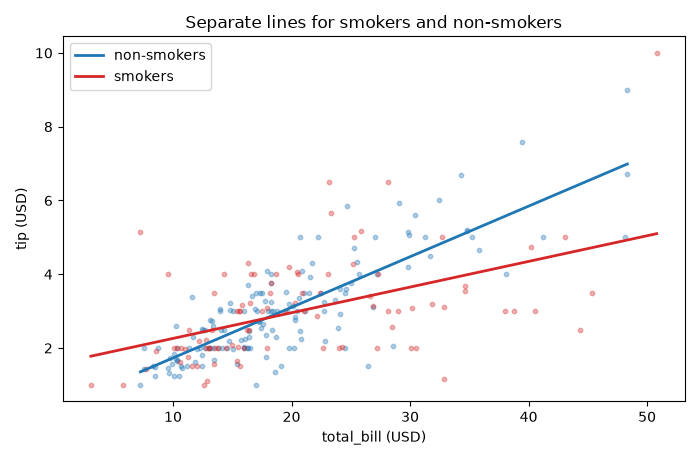
\includegraphics[width=0.92\linewidth]{fig_smoker.png}

    \vspace{-0.1em}
    {\scriptsize The smokers' line is flatter: tips rise more slowly with the bill.}

    \vspace{0.3em}
    \raggedright\small
    \key{Robust check:} with heteroskedasticity-robust (HC3) errors the slope
    difference is still significant, $P=0.008$ (ordinary: $3\times10^{-6}$).\par
  \end{column}
  \end{columns}
\end{frame}

% ===================== 9. OTHER QUALITATIVE AND SUMMARY =============
\begin{frame}{9. Other qualitative predictors, and what the data say}
  \begin{columns}[T]
  \begin{column}{0.52\textwidth}
    \small
    More than two classes: $c-1$ indicators, and their interactions with $X_1$
    give a slope per class. Same two tests, $\alpha=0.05$:

    \vspace{0.3em}
    {\scriptsize
    \begin{tabular}{@{}lrrrr@{}}
      \toprule
       & \multicolumn{2}{c}{equal slopes} & \multicolumn{2}{c}{identical} \\
       & $F^{*}$ & $P$ & $F^{*}$ & $P$ \\
      \midrule
      smoker (2) & $22.7$ & $3.3\times10^{-6}$ & $12.0$ & $1.1\times10^{-5}$ \\
      sex (2)    & $0.30$ & $0.58$  & $0.17$ & $0.85$ \\
      time (2)   & $2.10$ & $0.15$  & $1.05$ & $0.35$ \\
      day (4)    & $3.66$ & $0.013$ & $2.00$ & $0.066$ \\
      \bottomrule
    \end{tabular}}

    \vspace{0.2em}
    {\scriptsize df: $(1,240)$, $(2,240)$; for \texttt{day} $(3,236)$, $(6,236)$.}

    \vspace{0.2em}
    \begin{itemize}
      \item \key{Smoker} is the only grouping that changes the line; sex and
            time show nothing; \texttt{day} is borderline.
      \item The tests assume constant variance, which fails here (week~3); the
            HC3 check on smoker supports it.
    \end{itemize}
  \end{column}
  \begin{column}{0.48\textwidth}
    \small
    \key{What the tips data say}
    \begin{itemize}
      \item The bill explains $46\%$ of the variance of the tip; party size adds
            about $1$ point of $R^2$.
      \item No curvature and no bill\,$\times$\,size interaction.
      \item A predictor built from the others (bill per person) adds no fit and
            breaks the coefficients (VIF $>10$, size flips sign).
      \item Smokers' tips grow $0.070$ per dollar of bill, non-smokers' $0.137$.
    \end{itemize}

    \vspace{0.3em}
    \key{Caveats.} The variance grows with the bill and the residuals are not
    normal, so intervals for new tips are too narrow at high bills; a few
    high-leverage bills move the coefficients by $12$--$19\%$.
  \end{column}
  \end{columns}
\end{frame}

\end{document}
